%CONFIG DEL DOC
\documentclass[a4paper, 12pt, spanish]{article}
\usepackage[utf8x]{inputenc}
\usepackage{babel}
\usepackage{multicol, enumitem}
\usepackage{graphicx}
\graphicspath{ {images/} }
\usepackage{anysize} 

\marginsize{2.5cm}{2.5cm}{2cm}{2cm} 


\def\code#1{\texttt{#1}}


\title{Informe Trabajo Práctico N°2 \linebreak \textit{Atari Asteroids} \linebreak}

\author{Malena Díaz Falvo y Agustín Ormazábal}
\date{30 de Junio de 2019}

\begin{document}


\begin{figure}[t]
	
\includegraphics[width=8cm]{logoFIUBA} 
\end{figure}
\maketitle

\thispagestyle{empty}
\newpage

\setcounter{page}{2}
\pagestyle{plain}

\section*{Introducción}
El actual proyecto consta de la implementación de una reversión del juego
Asteroids en lenguaje ISO-C99 utilizando la biblioteca gráfica SDL2. Para su recreación
se implementó el concepto de TDA, entre otras funcionalidades, incorporados a lo largo
del curso. \newline
 
\section*{Desarrollo}
Para abordar este proyecto, se utilizaron y modificaron algunos de los archivos brindados para el TP1 (reversión del Lunar 
Lander). Además, se diseñaron y utilizaron diferentes TDAs para los objetos del juego, obteniendo finalmente los siguientes \texttt{.h}:

\begin{multicols}{2}
\begin{itemize}[label=$\bullet$]

	\item \texttt{caracteres.h}
	\item \texttt{config.h} 
	\item \texttt{dibujar.h}
	\item \texttt{diccionario.h}
	\item \texttt{movimiento.h}
	\item \texttt{nave.h}
	\item \texttt{asteroides.h}
	\item \texttt{disparos.h}
	\item \texttt{graficador.h}
	\item \texttt{iterador.h}
	\item \texttt{lista.h}
	

\end{itemize}
\end{multicols}
\medskip

\begin{figure}[h]
 	\centering
	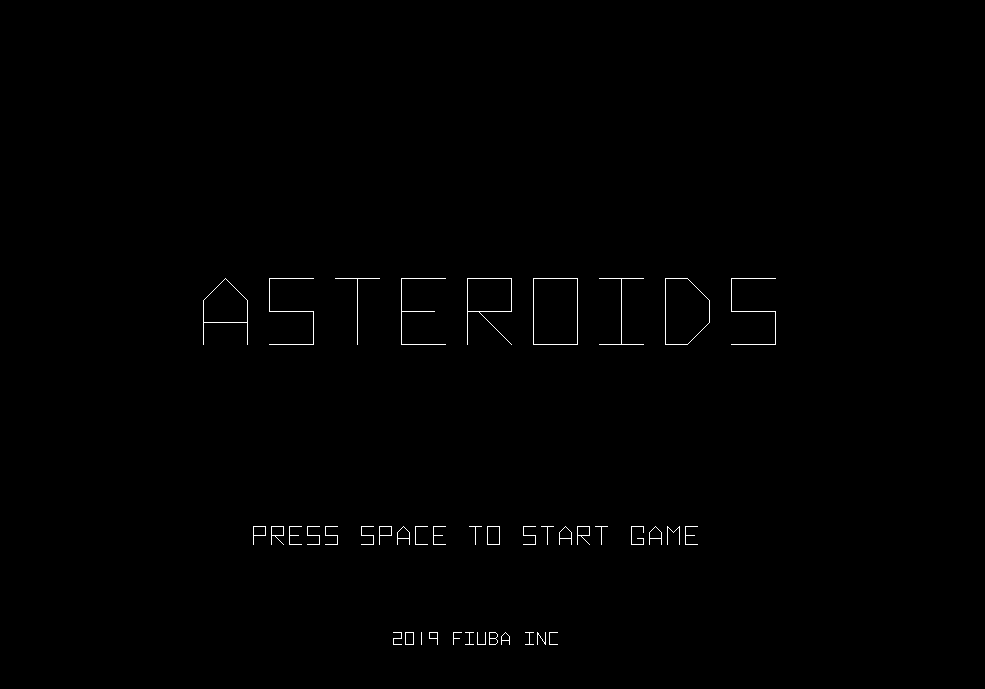
\includegraphics[width=12cm]{start_screen}
	\caption{Pantalla de inicio del juego.}
\end{figure}



\begin{figure}[h]
 	\centering
	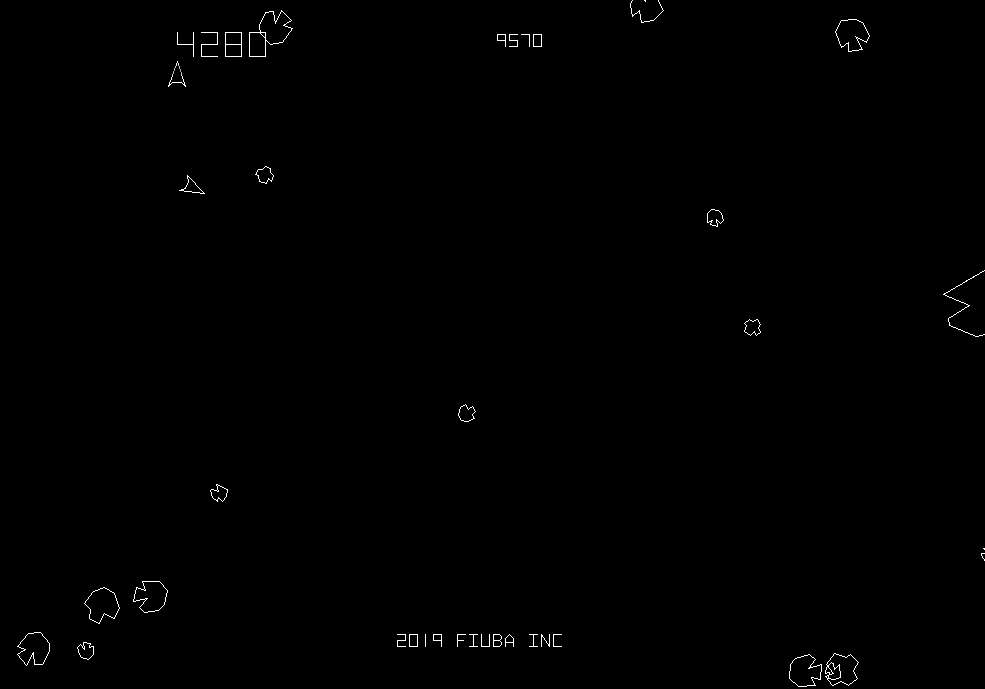
\includegraphics[width=12cm]{juego} 
	\caption{Partida en transcurso.}
\end{figure}

\begin{figure}[h]
 	\centering
	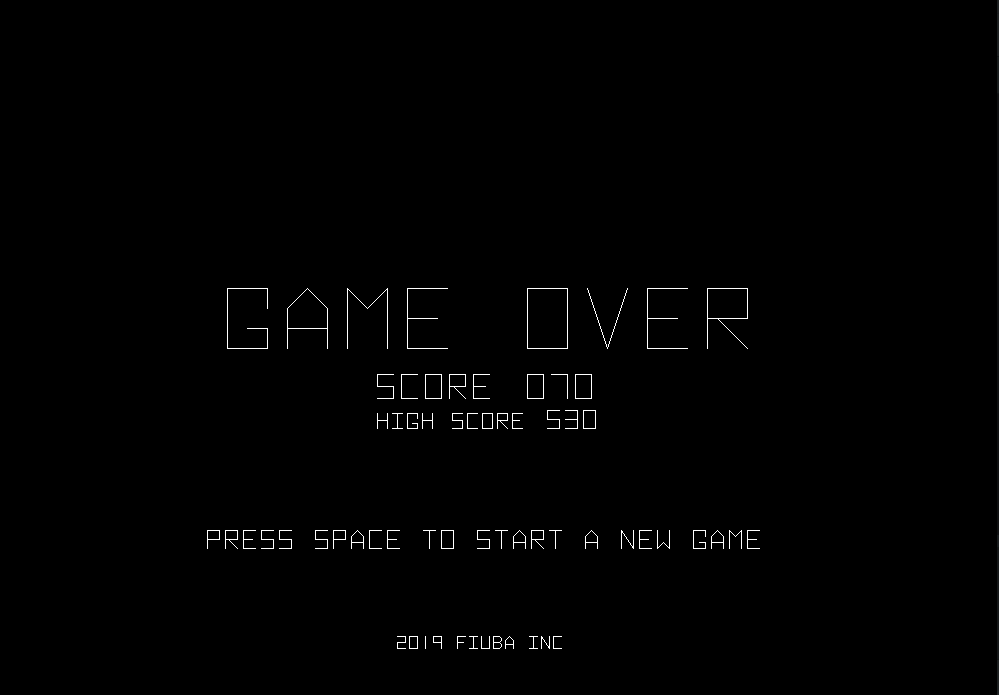
\includegraphics[width=12cm]{game_over_screen}
	\caption{Pantalla de finalización de la partida.}
\end{figure}


\section*{Dificultades}


\end{document}